\documentclass{beamer}
\usepackage[numbers]{natbib}

% \usepackage{beamerthemesplit} // Activate for custom appearance

\title{W4240/W6240 \\\qquad \\Data Mining/\\Statistical Machine Learning}
\author{Frank Wood}
\date{\today}

\newcommand{\comment}[1]{}


\def\x{\mathbf{x}}
\def\transpose{T}
\def\bmu{\boldsymbol{\mu}}

\def\x{\mathbf{x}}
\def\t{\mathbf{t}}
\def\y{\mathbf{y}}










\newcommand{\ponedec}{\mathcal{P}^\downarrow_1}
\newcommand{\pone}{\mathcal{P}_1}
\newcommand{\rank}[1]{\mathrm{RANK}\left[#1\right]}
\newcommand{\E}[1]{\mathrm{E}\left[#1\right]}
\newcommand{\py}{\mathcal{PY}}
\newcommand{\iid}{iid.}
\newcommand{\drawiid}{\stackrel{\text{iid}}{\sim}}
\newcommand{\vect}[1]{\mathbf{#1}}
\newcommand{\indicator}[1]{\text{I}\left[ #1 \right]}
\newcommand{\pdcoag}{PD(d_1,0)-\text{COAG}}
\newcommand{\todo}{\textbf{*TODO*}}
\newcommand{\igram}{\text{$\infty$-gram}}
\newcommand{\Prob}{\text{P}}

\def\mm{sequence memoizer }
\def\MM{SM }

\def\pibf{{\boldsymbol{\pi}}}
\def\Pibf{{\boldsymbol{\Pi}}}
\def\Thetabf{{\boldsymbol{\Theta}}}
\def\thetabf{{\boldsymbol{\theta}}}

\def\kapbf{\boldsymbol{\kappa}}
\def\taubf{\boldsymbol{\tau}}
\def\thebf{\boldsymbol{\theta}}
\def\rhobf{\boldsymbol{\rho}}
\def\phibf{\boldsymbol{\phi}}
\def\pbf{\mathbf{p}}
\def\qbf{\mathbf{q}}
\def\sbf{\mathbf{s}}
\def\tbf{\mathbf{t}}
\def\ybf{\mathbf{y}}
\def\wbf{\mathbf{w}}
\def\xbf{\mathbf{x}}
\def\zbf{\mathbf{z}}
\def\rbf{\mathbf{r}}
\def\tbf{\mathbf{t}}
\def\kbf{\mathbf{k}}
\def\Xbf{\mathbf{X}}
\def\0bf{\mathbf{0}}
\def\Ibf{\mathbf{I}}
\def\phibf{\mathbf{\phi}}
\def\Phibf{\mathbf{\Phi}}
\def\disteq{{\stackrel{D}{=}}}
\def\EE{{\mathbb{E}}}

\def\phiv{\varphi}
\def\phivbf{\boldsymbol{\varphi}}

\def\Ocal{\mathcal{O}}

\DeclareMathOperator*{\Bet}{Beta}
\DeclareMathOperator{\coag}{COAG}
\DeclareMathOperator{\frag}{FRAG}
\DeclareMathOperator*{\rnk}{RANK}
\DeclareMathOperator*{\gem}{GEM}
\DeclareMathOperator*{\pd}{PD}
\DeclareMathOperator*{\gd}{GDir}
\DeclareMathOperator*{\Dir}{Dir}
\DeclareMathOperator*{\Discrete}{Discrete}
\DeclareMathOperator*{\Mult}{Multinomial}


\begin{document}

\frame[t]{\titlepage}

%\section[Outline]{}
%\frame[t]{\tableofcontents}

\section{Introduction}
\subsection{Overview of Topics}

\section{}
\subsection{}

\frame[t] { 
\frametitle{Introduction}
\begin{itemize}
\item Data mining is the search for patterns in large collections of data
\begin{itemize}
\item Designing models
\item Fitting models to data
\item Using models to perform inference/prediction
\end{itemize}
\item Pattern recognition is concerned with {\em automatically} finding patterns in data / learning models
\item Machine learning is pattern recognition with concern for computational tractability and full automation
\item Data mining = Machine Learning = Applied Statistics
\begin{itemize}
\item Scale
\item {\em Computation}
\end{itemize}

\end{itemize}
}

\frame[t] { 
\frametitle{High Level Course Goals}
\begin{itemize}
\item Problem formulation
\begin{itemize}
\item Starting from data and/or a question, you will learn how to create and design a model that will answer the question(s) of interest.
\item You will learn how to formally, mathematically codify a model.
\item You will learn how to fit models.
\item You will learn to think about computational/inferential trade-offs.
\end{itemize}
\item Tool {\em Creation}
\begin{itemize}
\item You will learn how to design and implement general purpose learning algorithms
\item You will implement inference algorithms for several models such as latent Dirichlet allocation, Bayesian logistic regression, Gaussian mixture models and more.
\end{itemize}
\item Practice
\begin{itemize}
\item Through your homework and final project you will be evaluated on how well you can put into practice the theory that will be taught in class.
\end{itemize}

%\begin{itemize}
%\item Scale
%\item {\em Computation}
%\end{itemize}

\end{itemize}
}

\frame[t] { 
\frametitle{Style of Instruction}
\begin{itemize}
\item Great textbook (Bishop, Pattern Recognition and Machine Learning, {\em required!})!
\begin{itemize}
\item Will follow second half of text closely.
\end{itemize}
\item Class time will be spent on {\em theory} and ``{\em proof},'' explaining the tricky parts of the text by doing math on the board.
\item Homework (extensive and hard) will be spent on practice.
\item Team-based final project
\item This is {\em not} a {\em ``What tool do we use and how do we use it?''}  course!
%\begin{itemize}
%\item Scale
%\item {\em Computation}
%\end{itemize}

\end{itemize}
}

\frame[t] { 
\frametitle{Grading - What you should expect.}
\begin{figure}[htbp]
\begin{center}
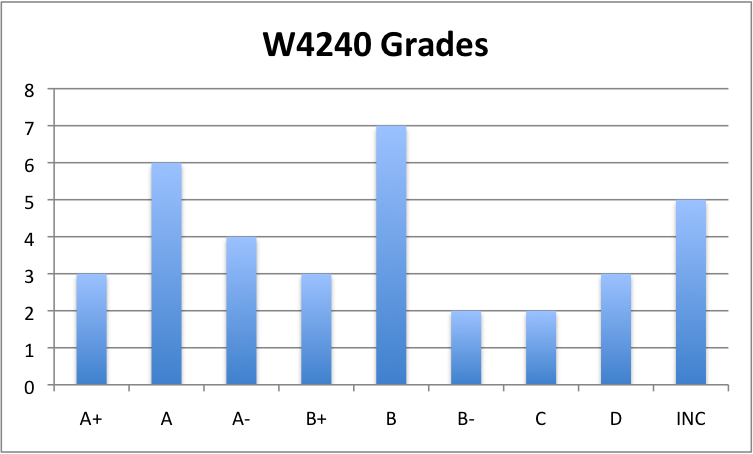
\includegraphics[width=11cm]{grad_dist}
\caption{Fall 2010 Grade Distribution}
\label{default}
\end{center}
\end{figure}

}

\frame[t] { 
\frametitle{Links and Syllabus}
\begin{itemize}
\item 	Course home page :  \href{http://www.stat.columbia.edu/~fwood/w4240/}{http://www.stat.columbia.edu/$\sim$fwood/w4240/}
	\item {\em Bookmark} this page (not courseworks)
	\item Guest lectures may be sprinkled throughout the course.
\end{itemize}	
 	}

\frame[t] { 
\frametitle{Prerequisites}
\begin{itemize}
\item Linear algebra
\item Multivariate calculus (matrix and vector calculus)
\item Probability and statistics at a masters level
\item Programming experience in some language like pascal, matlab, c++, java, c, fortran, scheme, etc.
\item Some algorithmic complexity theory (basics) useful
\item Information theory (entropy, KL-divergence)
\end{itemize}
}

\frame[t] { 
\frametitle{Review}
Good idea to familiarize yourself with PRML \cite{Bishop2006} Chapter 1 and 2 and Appendices B,C,D, and E.
In particular:
\begin{itemize}
\item Information theory
\item Multivariate Gaussian distribution
\item Discrete, multinomial, and Dirichlet distributions
\item Lagrange multipliers
\item Matlab
\end{itemize}

We will offer extra Matlab programming sections, a review of both the multivariate Gaussian and information theory.


}

\frame[t] { 
\frametitle{Homework (from anonymous student feedback)}

\begin{quote}
The assignments were challenging and probably the best part of the course. It was with bated breath, and nervous anticipation - almost like a blind date with someone you knew would be pretty - that we waited for the homework� ok, maybe that was 10\% exaggerated. ....
\end{quote}
\begin{quote}
The assignments in this course were more challenging than any other course I have taken in the past.
\end{quote}
\begin{quote}
Really enjoyed the assignments in this class. Excellent job putting them together.
\end{quote}
\begin{quote}
Very difficult programming assignments, and I learned a lot doing them, �
\end{quote}
The homework in this course is {\em programming}.  You will {\em implement} various data mining / machine learning algorithms.  If you have not programmed before the course is doable but difficult.  
}

\frame[t] { 
\frametitle{Project}
The final project is a semester-long, significant piece of team-based work that demonstrates your data mining / statistical machine learning knowledge on a problem domain of interest to you (and hopefully also of interest to a larger academic, governmental, or industry community). The deliverables include a 2-3 page proposal; a short, publication-quality paper; and a 10-20 minute presentation.
}



\frame[t] { 
\frametitle{Syllabus}
\begin{itemize}
\item Review
\item Graphical models
\begin{itemize}
\item Belief propagation
\end{itemize}
\item Expectation Maximization
\item Variational Inference
\item Sampling
\item Misc.
\end{itemize}
Along the way you will implement estimation and inference procedures for the following models (minimally)
\begin{itemize}
\item Gaussian mixture model
\item Bayesian linear regression
\item Bayesian logistic regression
\item Latent Dirichlet allocation
\item ...
\end{itemize}

}

\frame[t] { 
\frametitle{Past Example Projects}
See website for links to related talks.
}


	\bibliographystyle{plainnat}
	\begin{frame}[t,allowframebreaks]{Bibliograpy}

\bibliography{../../../../../papers/uber.bib}
\end{frame}



\end{document}